\documentclass[10pt,a4paper]{article}
\usepackage{amsmath}
\usepackage{amsfonts}
\usepackage{amssymb}
\usepackage{graphicx}
\usepackage[french]{babel}
\usepackage[T1]{fontenc}
\usepackage[utf8x]{inputenc}
\graphicspath{{images/}}
\usepackage{parskip}
\usepackage{fancyhdr}
\usepackage{vmargin}
\setmarginsrb{3 cm}{2.5 cm}{3 cm}{2.5 cm}{1 cm}{1.5 cm}{1 cm}{1.5 cm}

\title{Défis en Intelligence Artificielle}                             % Title
\author{Maxime De Wolf\\
		Dimitri Waelkens}                               % Author
\date{\today}                                           % Date

\makeatletter
\let\thetitle\@title
\let\theauthor\@author
\let\thedate\@date
\makeatother

\pagestyle{fancy}
\fancyhf{}
\rhead{\theauthor}
\lhead{\thetitle}
\cfoot{\thepage}

\begin{document}
   	
   	%%%%%%%%%%%%%%%%%%%%%%%%%%%%%%%%%%%%%%%%%%%%%%%%%%%%%%%%%%%%%%%%%%%%%%%%%%%%%%%%%%%%%%%%%
   	
   	\begin{titlepage}
   		\centering
   		\vspace*{0.5 cm}
   		
\includegraphics[scale = 0.75]{UMONS}\\[1.0 cm]   % University Logo
   		\textsc{\LARGE Université de Mons}\\[2.0 cm]   % University Name
   		\textsc{\large TP4}\\[0.5 cm]               % Course Name
   		\rule{\linewidth}{0.2 mm} \\[0.4 cm]
   		{ \huge \bfseries \thetitle}\\
   		\rule{\linewidth}{0.2 mm} \\[1.5 cm]
   		
   		\begin{minipage}{0.4\textwidth}
   			\begin{flushleft} \large
   				\emph{Auteur:}\\
   				\theauthor
   			\end{flushleft}
   		\end{minipage}~
   		\begin{minipage}{0.4\textwidth}
   			\begin{flushright} \large
   				\emph{}                                  % Your Student Number
   			\end{flushright}
   		\end{minipage}\\[2 cm]
   		
   		{\large \thedate}\\[2 cm]
   		
   		\vfill
   		
   	\end{titlepage}
   	
   	%%%%%%%%%%%%%%%%%%%%%%%%%%%%%%%%%%%%%%%%%%%%%%%%%%%%%%%%%%%%%%%%%%%%%%%%%%%%%%%%%%%%%%%%%
   	
   	\section{Configuration de \textit{Cartographer}}
	
	
		La configuration de cartographer est réalisée via son fichier de configuration : uafr_cartographer.lua. Dans ce fichier nous avions modifier trois paramêtres :
		
			\begin{itemize}
			
			\item num_accumulated_range_data définit le nombre de messages requis pour reconstruire un scan complet (une image de l'espace autour du robot en temps t) en augmentant cette variable nous augmentons la précision d'un scan.
			\item num_subdivisions_per_laser_scan défini le nombre de points utiliser par scan. C'est point sont ensuite utilisées pour reconstituer la carte. Augmenter ce nombre de points permet à cartographer de mieux reconstituer une sous-carte.
			The size of submaps is configured through
			\item TRAJECTORY_BUILDER_2D.submaps.num_range_data conrespond à la taille de sous carte. Ce paramètre doit être plus grand que num_accumulated_range_data.
			
			\end{itemize}
			
		Augmenter ces paramètres permet augmenter la qualité de la carte calculée. Nous avions initialisé ses trois paramètres à 200. Et nous avions obtenu le résultat suivant :
		
		\begin{figure}[h]
   			\begin{center}
   				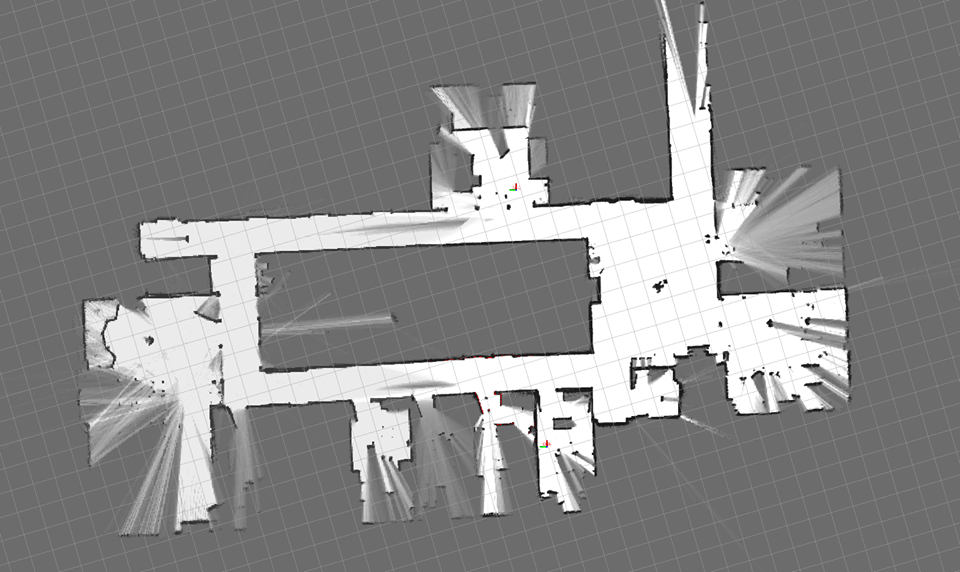
\includegraphics[width=0.75\linewidth]{map}
   			\end{center}
   			\caption{Carte obtenue grâce à \textit{Cartographer}}
   			\label{fig:map}
   		\end{figure}

		Ce résultat est assez bon. Chaque pièce est bien reconstituer, modulo les meubles qui permettent pas de réaliser une représentation complète de chacune des pièces. Aucune pièce chevauche une autre. De plus les mur et les angles sont bien droit. Augmenter au-delà permutera pas d'améliorer sensiblement le résultat et risque de causée de la latence à cause de calculs inutiles 
   	
   
   	\section{Localisation des objets}
   	
   		Cette section présente les résultats obtenus pour la détection d'objets que le robot à filmé. Nous expliquons donc dans un premier temps la logique que nous avons suivies pour obtenir ces résultats. Nous justifions ensuite la manière dont ils pourraient être améliorés.
   		
   		\subsection{Technique utilisée}
   		
   			Pour résoudre ce problème, nous utilisons une technique très simple. Effectivement, à chaque fois que le robot détecte un objet, nous repérons la position du robot ainsi que la distance à laquelle l'objet à été filmé. Cependant, nous avons également besoin de l'orientation du robot pour calculer la position de l'objet.
   			
   			Afin d'avoir l'orientation du robot, nous repérons également l'emplacement précédent duquel le robot voyait également cet objet. Nous pouvons donc calculer former par la droite passant par ces deux points dans le repère.
   			
   			Ensuite, grâce à la distance de l'objet filmé, nous pouvons déterminer la position de celui-ci.\\
   			
   			Le robot travaille sur un grand nombre d'image similaire. Nous calculons donc plusieurs fois la position du même objet.
   			
   			Pour pallier à ce problème nous utilisons un algorithme de \textit{clustering} simple afin de regrouper les position qui sont susceptible de représenter un même objet.
   			
   			Cette algorithme fonctionne de la manière suivante:
   			\begin{enumerate}
   				\item Pour chaque position, un regarde si elle est proche du centre d'un \textit{cluster} existant;
   				\item Si c'est le cas, on l'ajoute à ce \textit{cluster};
   				\item Sinon, on crée un nouveau \textit{cluster} qui contient cette position;
   			\end{enumerate}
   		
   			Finalement pour retrouver la position de chaque objet, on calcule le centre de chaque \textit{cluster}. Cette technique nous donne les résultats exposés par la Table \ref{tab:res}.
   	
   		\begin{table}[h]
   			\begin{center}
   				\begin{tabular}{|c|c|c|}
   					\hline
   					Objet & Position 1 & Position 2\\
   					\hline
   					\textit{teddy bear} & (2.399926850060335, -0.008283207609849293)& (12.604331235659147, 14.238862468344005) \\
   					\hline
   					\textit{motorbike} & (8.366541118657906, 14.943175542227172) & / \\
   					\hline
   					\textit{backpack}& (4.832979494372698, 2.7004257263585636) & / \\
   					\hline
   					\textit{suitcase} & (5.446312729568893, 16.221012094608028) & / \\
   					\hline
   					\textit{pottedplant} & (12.343678479509247, 14.322766597693517) & (0.9148871784197752, 23.25876369786711) \\
   					\hline
   					\textit{stop sign} & (7.87594829417553, 15.93296178462322) & / \\
   					\hline
   					\textit{refrigerator} & (6.239195085908132, 13.789541846887905) & / \\
   					\hline
   				\end{tabular}
   			\end{center}
   			\caption{Positions obtenues pour chaque objet détecté}
   			\label{tab:res}
   		\end{table}
   	
   		\subsection{Discussion sur les résultats}
   		
   		Grâce à la Table \ref{tab:res}, nous pouvons voir que nos résultats sont assez mauvais par rapport aux résultats attendus car nous ne détectons pas le bon nombre d'objets. Nous dressons donc une liste non-exhaustive de tous les facteurs qui pourraient être responsables.\\
   		
%   			todo: position via 2 positions

		Pour retrouver la position du robot précédant la détection de l'objet, nous prenons la position du robot durant la détection précédente d'un objet. Cela implique que nous prenons éventuellement la position du robot pendant la détection d'un autre objet. Cela peut donc causer la création de \textit{clusters} artificiel.
		
		Une solution pour régler ce problème est de tester si l'objet précédemment détecté est le même que celui en cours de détection. On pourrait notamment faire ceci en se basant sur la technique de \textit{clustering} que nous avons utilisé.
		
		Une autre solution serait de ne plus prendre la position du robot pendant la détection de l'objet précédent mais de sélectionner la position du robot juste avant de détecter l'objet. Cette solution est selon nous la plus logique à appliquer.\\

		Notre technique de \textit{clustering} est très (trop ?) simple. Dès lors, on peut se demander si d'autres techniques donneraient de meilleurs résultats. Effectivement, chaque position que nous trouvons découle de la formation d'un \textit{cluster}. Un problème à ce niveau aurait donc des conséquences directes sur nos résultats au niveau du nombre d'objets détectés.\\

   		Le robot nous fourni la distance à laquelle se trouve ce qu'il voit. Cependant, il arrive qu'il détecte plusieurs objets sur la même image. Dans ce cas nous utilisons la même distance sur tous ces objets ce qui implique que tous les objets présents sur une même image auront d'office la même position. Or, cela est loin d'être vrai. Ce problème influe donc sur la position des objets détectés, ce qui a une incidence sur les \textit{clusters} formés et donc sur les résultats finaux.
   
   	%\bibliographystyle{plain}
   	%\bibliography{biblist}
          	
\end{document}
